\clearpage

\chapter{Limits cross checks and additional plots}
\label{appendix:limit}

During the limit derivation, the systematic uncertainties (translated in term of nuisance parameter) are fitted to the data,
several checks are have been performed to ensure the quality of our statistical model.
If some of the nuisance parameters are significantly different from their nominal value 
(ie before fit), it can be symptomatic of an important mis-modelling and must be carefully scrutinised.
Also the correlation between the nuisance parameter and the signal strength (which reflects the degeneracy of the fit) 
is an important element to keep under control, in fact it reflects how well the data can constraint the nuisance parameters.
Finally, to have a feeling of the behaviour of the likelihood at its minimum one can check 
the negative log likelihood profile in each nuisance parameter direction. 
We performed all this checks using the package NuisanceCheck-00-00-05 described in \cite{NPcheck}.

The signal and background model with the signal normalisation free (unconditional fit) is fitted to the data,
in the following example plots the signal is assumed for the mass point mA~=~120 GeV, tan$\beta$~=~20,  
The difference between the post fit and pre-fit value of the nuisance parameter along with their errors is shown in figure~\ref{fig:np_pull_veto}-\ref{fig:np_pull_comb},
respectively for the b-veto, b-tag channel and the combination between them.
Figure~\ref{fig:np_correlation_veto}-\ref{fig:np_correlation_comb} shows the correlation matrix between the nuisance parameters respectively for
the veto category, tag category and the combination between the two channels.
Figure~\ref{fig:llh_1}-\ref{fig:llh_3} shows the behaviour of the likelihood at its minimum for 
each of the nuisance parameters (while a nuisance parameter is investigated the other are kept constant) for the combination between the channels.

%%%%%%%%%%%%%%%%%%%%%%%%%%%%%%%%%%%%%%%%%%%%%%% PULLS %%%%%%%%%%%%%%%%%%%%%%%%%%%%%%%%%%%%%%%%%%%%%%%%%%%%%%%%%%
\begin{figure}[htp]
     \begin{center}

            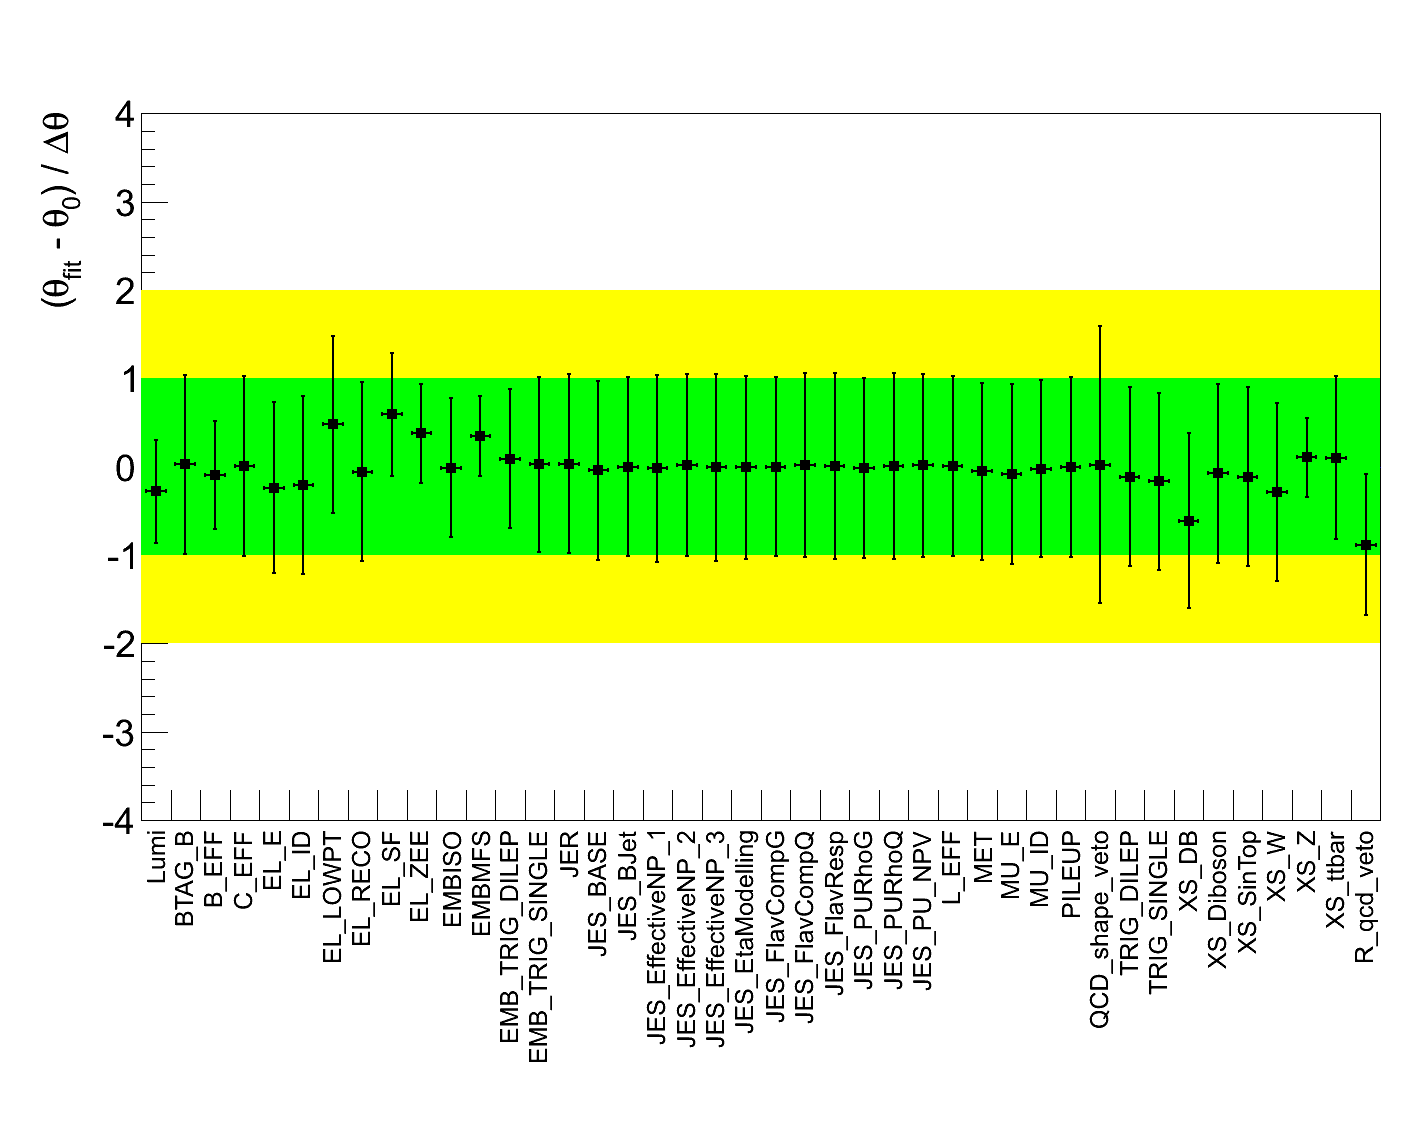
\includegraphics[width=\textwidth]{figure/np_check/pull_veto.png}
    \end{center}
    \caption{ Pulls for nuisance parameter considered in the fit,  mA = 120 GeV, tan$\beta$ = 20, for the veto channel.} 
    \label{fig:np_pull_veto}
\end{figure}


\begin{figure}[htp]
     \begin{center}

            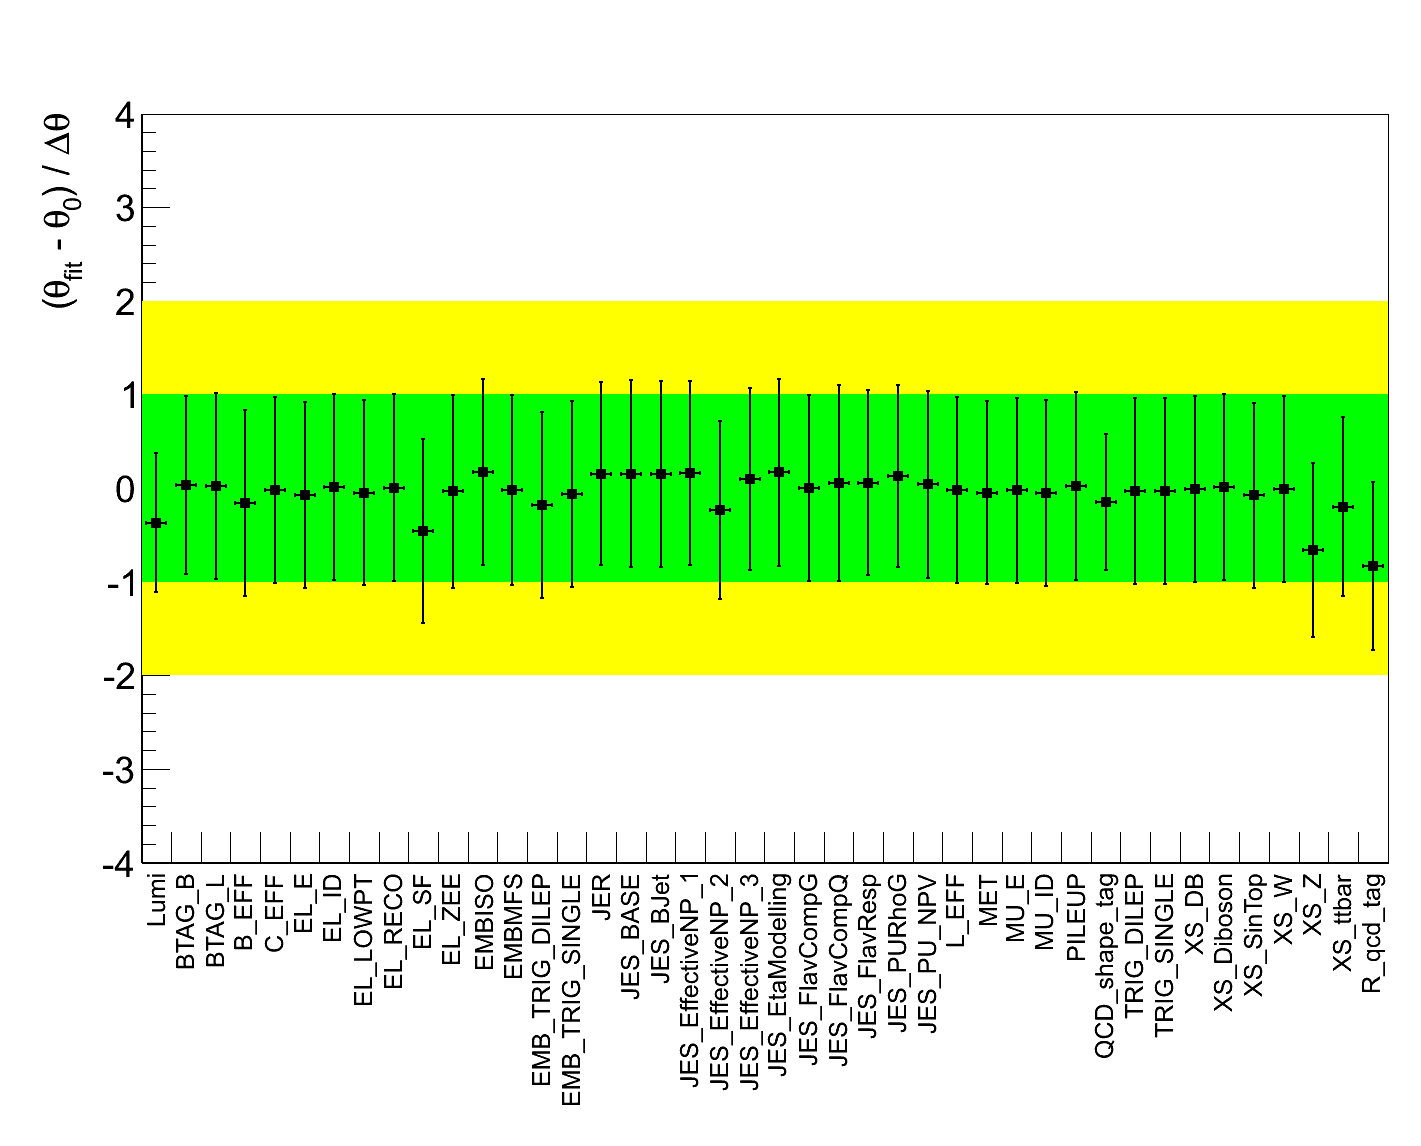
\includegraphics[width=\textwidth]{figure/np_check/pull_tag.png}
    \end{center}
    \caption{ Pulls for nuisance parameter considered in the fit,  mA = 120 GeV, tan$\beta$ = 20, for the tag  channel.} 
    \label{fig:np_pull_tag}
\end{figure}


\begin{figure}[htp]
     \begin{center}

            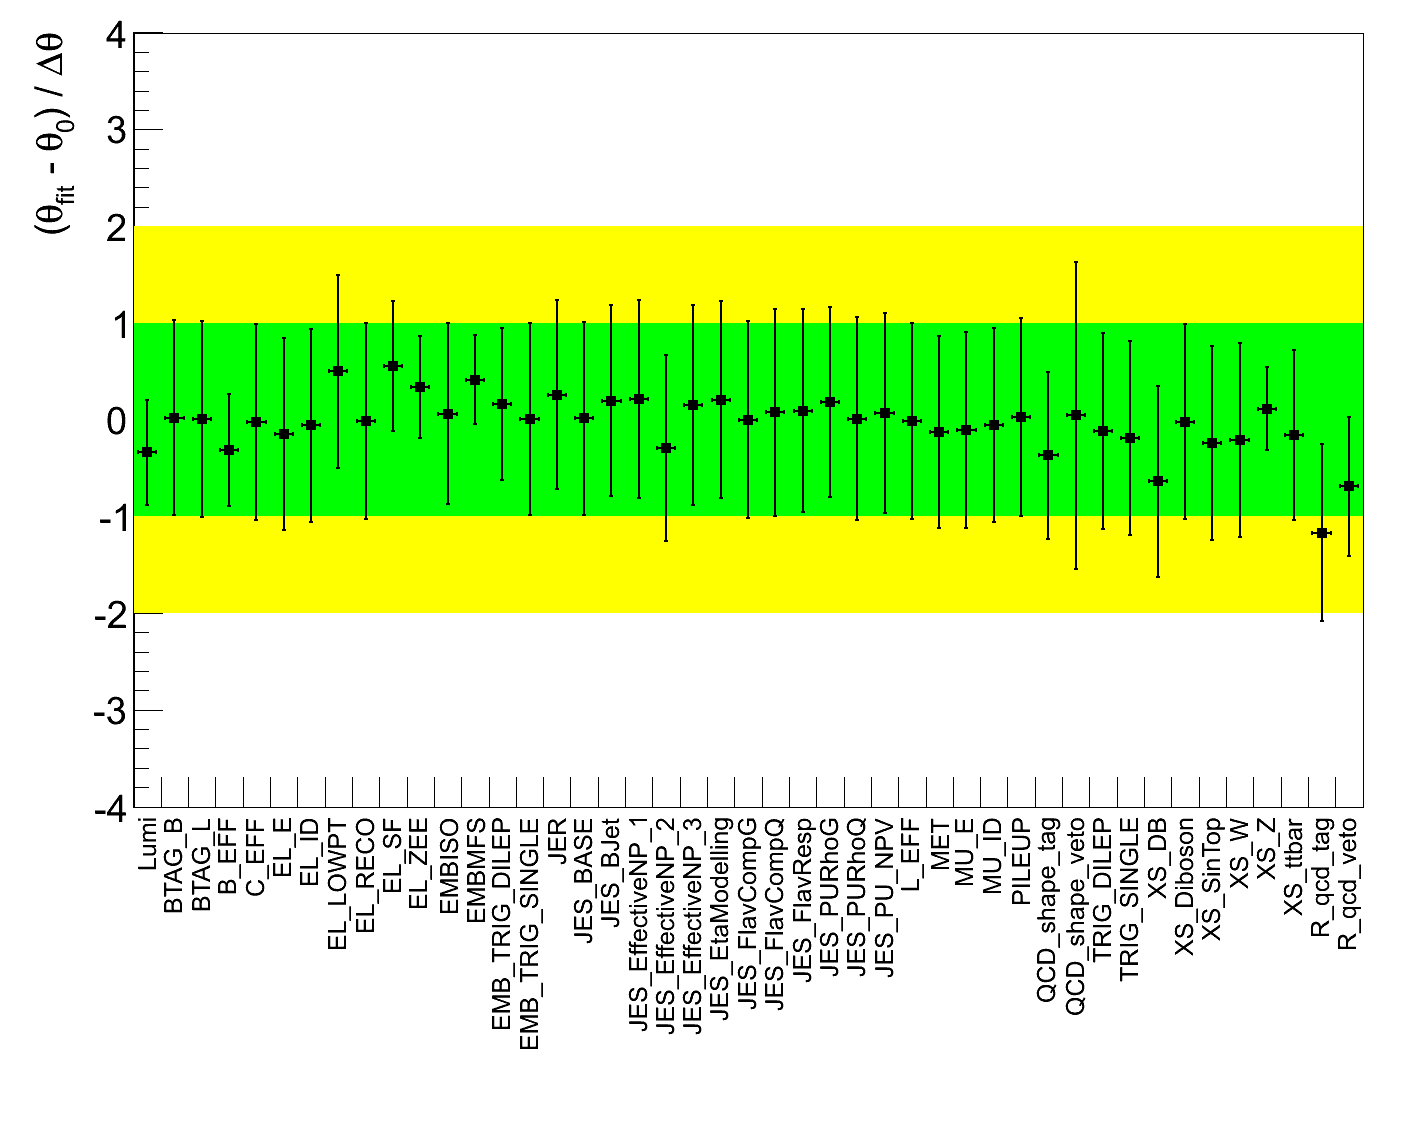
\includegraphics[width=\textwidth]{figure/np_check/NP_combined.png}
    \end{center}
    \caption{ Pulls for nuisance parameter considered in the fit,  mA = 120 GeV, tan$\beta$ = 20, combination between the two channel.} 
    \label{fig:np_pull_comb}
\end{figure}
%%%%%%%%%%%%%%%%%%%%%%%%%%%%%%%%%%%%%%%%%%%%%%%  %%%%%%%%%%%%%%%%%%%%%%%%%%%%%%%%%%%%%%%%%%%%%%%%%%%%%%%%%%

%%%%%%%%%%%%%%%%%%%%%%%%%%%%%%%%%%%%%%%%%%%%%%% CORRELATION MATRIX %%%%%%%%%%%%%%%%%%%%%%%%%%%%%%%%%%%%%%%%%%%%%%%%%%%%%%%%%%


\begin{figure}[htp]
     \begin{center}

           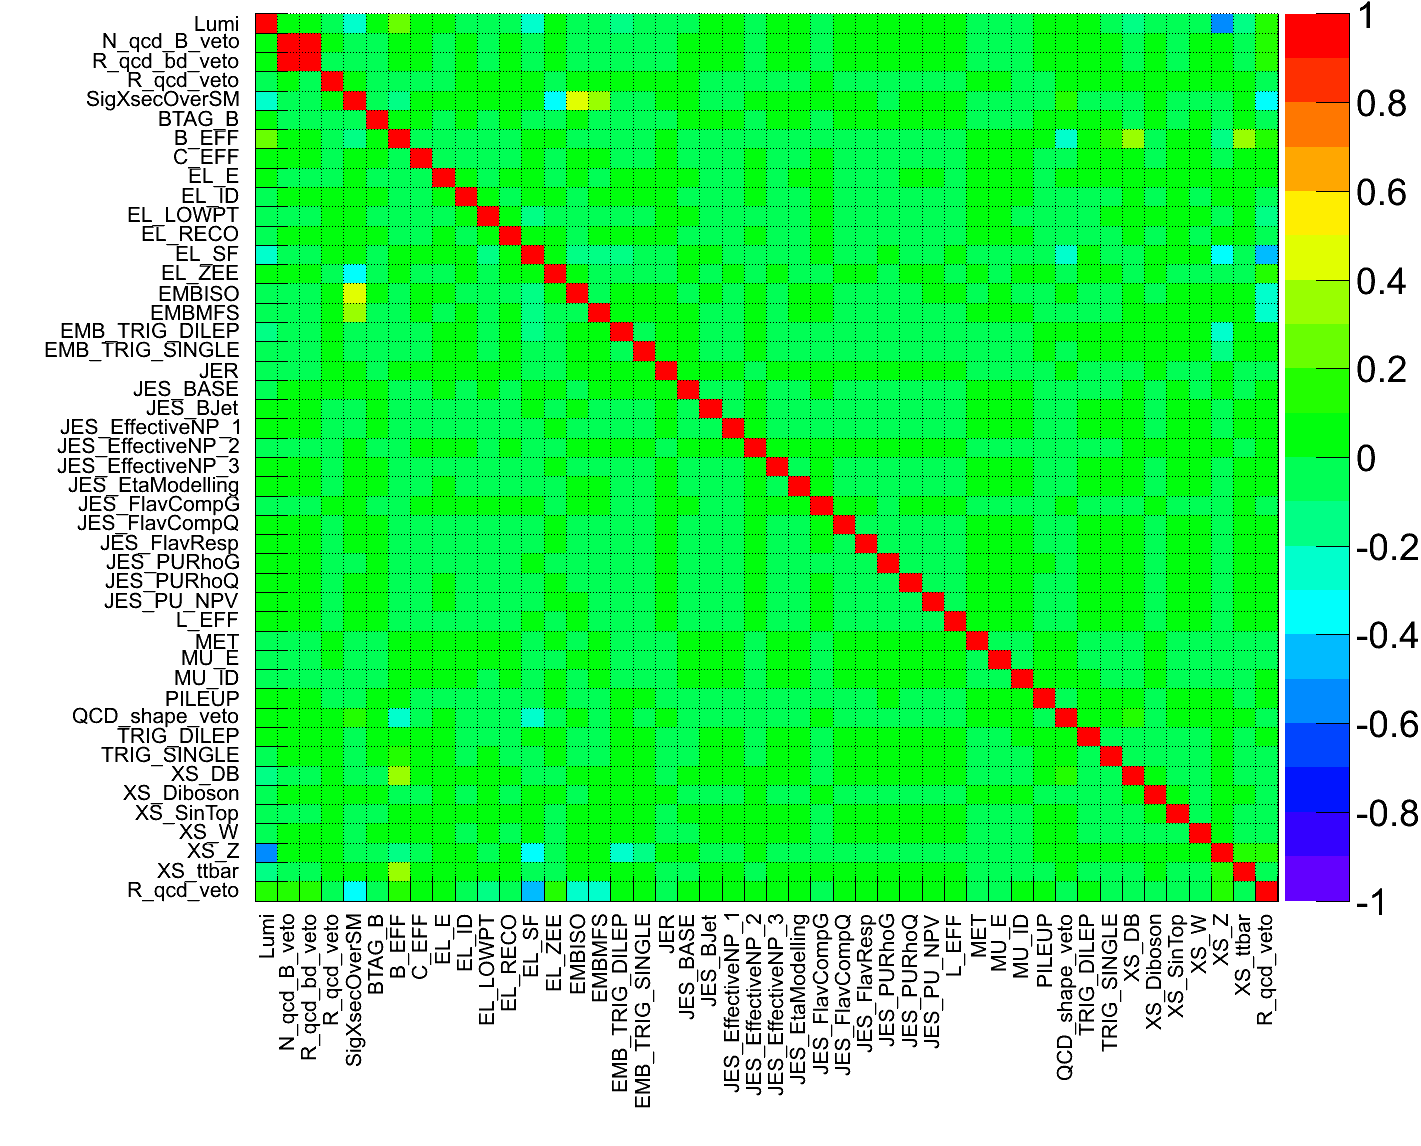
\includegraphics[width=\textwidth]{figure/np_check/matrix_veto.png}
    \end{center}
    \caption{ Correlation matrix for nuisance parameters considered in the fit. The point mA = 120 GeV and tan$\beta$ = 20 is considered for the tag channel.} 
    \label{fig:np_correlation_veto}
\end{figure}
\begin{figure}[htp]
     \begin{center}

           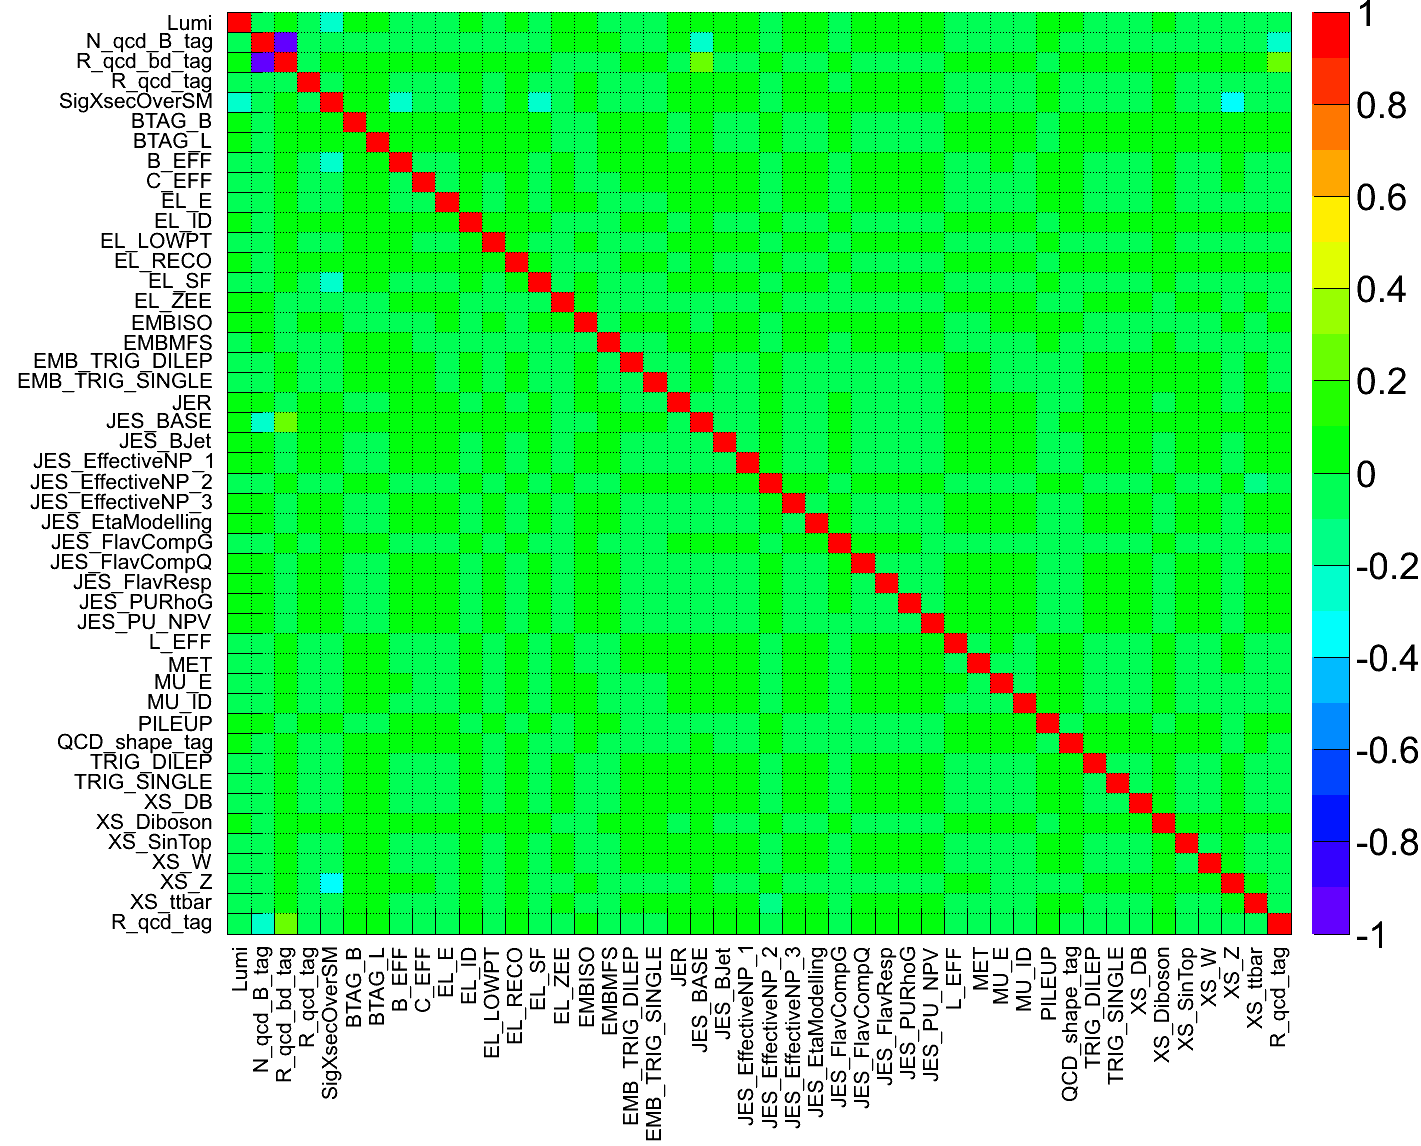
\includegraphics[width=\textwidth]{figure/np_check/matrix_tag.png}
    \end{center}
    \caption{ Correlation matrix for nuisance parameters considered in the fit. The point mA = 120 GeV and tan$\beta$ = 20 is considered for the tag channel.} 
    \label{fig:np_correlation_tag}
\end{figure}

\begin{figure}[htp]
     \begin{center}

           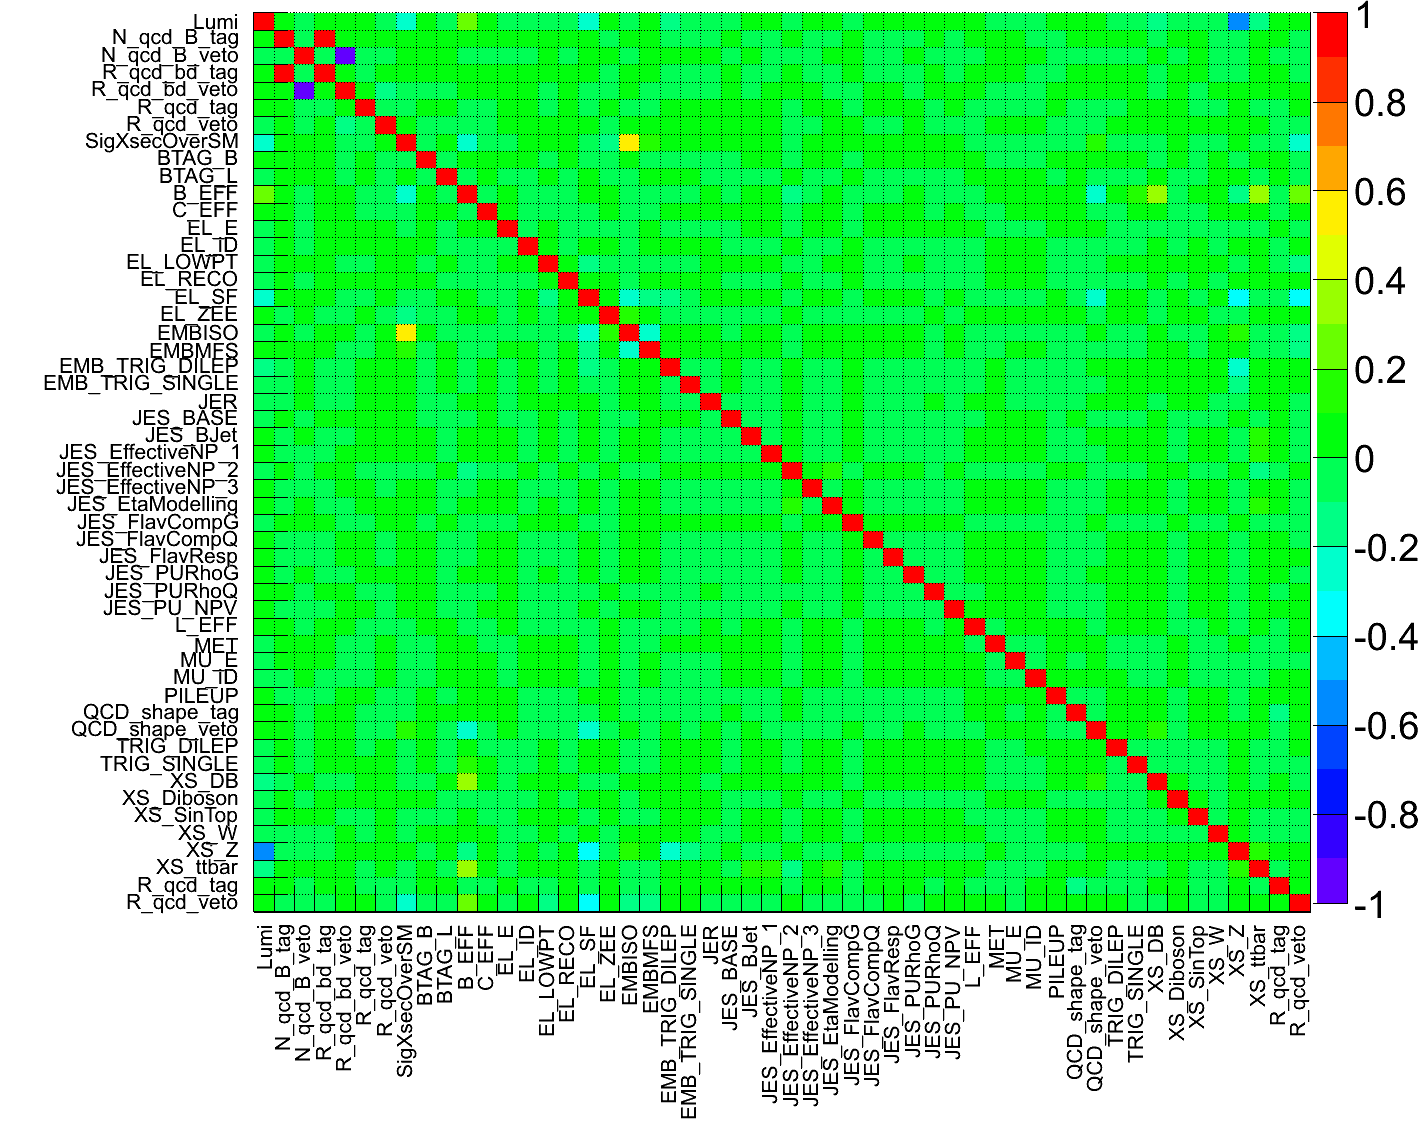
\includegraphics[width=\textwidth]{figure/np_check/comb_unconditiona_matrixl.png}
    \end{center}
    \caption{ Correlation matrix for nuisance parameters considered in the fit.  The point mA = 120 GeV and tan$\beta$ = 20 is considered for the combination of the b-tag and b-veto channels.} 
    \label{fig:np_correlation_comb}
\end{figure}
%%%%%%%%%%%%%%%%%%%%%%%%%%%%%%%%%%%%%%%%%%%%%%%  %%%%%%%%%%%%%%%%%%%%%%%%%%%%%%%%%%%%%%%%%%%%%%%%%%%%%%%%%%

%%%%%%%%%%%%%%%%%%%%%%%%%%%%%%%%%%%%%%%%%%%%%%% llh SCANS %%%%%%%%%%%%%%%%%%%%%%%%%%%%%%%%%%%%%%%%%%%%%%%%%%%%%%%%%%

\begin{figure}[htp]
     \begin{center}

            \includegraphics[page=8,width=0.3\textwidth]{figure/np_check/comb_LLHscan.pdf}
            \includegraphics[page=9,width=0.3\textwidth]{figure/np_check/comb_LLHscan.pdf}
            \includegraphics[page=10,width=0.3\textwidth]{figure/np_check/comb_LLHscan.pdf}\\
            \includegraphics[page=11,width=0.3\textwidth]{figure/np_check/comb_LLHscan.pdf}
            \includegraphics[page=12,width=0.3\textwidth]{figure/np_check/comb_LLHscan.pdf}
            \includegraphics[page=13,width=0.3\textwidth]{figure/np_check/comb_LLHscan.pdf}\\
            \includegraphics[page=14,width=0.3\textwidth]{figure/np_check/comb_LLHscan.pdf}
            \includegraphics[page=15,width=0.3\textwidth]{figure/np_check/comb_LLHscan.pdf}
            \includegraphics[page=16,width=0.3\textwidth]{figure/np_check/comb_LLHscan.pdf}\\
            \includegraphics[page=17,width=0.3\textwidth]{figure/np_check/comb_LLHscan.pdf}
            \includegraphics[page=18,width=0.3\textwidth]{figure/np_check/comb_LLHscan.pdf}
            \includegraphics[page=19,width=0.3\textwidth]{figure/np_check/comb_LLHscan.pdf}\\
            \includegraphics[page=20,width=0.3\textwidth]{figure/np_check/comb_LLHscan.pdf}
            \includegraphics[page=21,width=0.3\textwidth]{figure/np_check/comb_LLHscan.pdf}
            \includegraphics[page=22,width=0.3\textwidth]{figure/np_check/comb_LLHscan.pdf}\\

    \end{center}
    \caption{ Likelihood scans for nuisance parameter considered in the fit, mA = 120 GeV, tan$\beta$ = 20, combination between the two channel.} 
    \label{fig:llh_1}
\end{figure}

\begin{figure}[htp]
     \begin{center}

            \includegraphics[page=23,width=0.3\textwidth]{figure/np_check/comb_LLHscan.pdf}
            \includegraphics[page=24,width=0.3\textwidth]{figure/np_check/comb_LLHscan.pdf}
            \includegraphics[page=25,width=0.3\textwidth]{figure/np_check/comb_LLHscan.pdf}\\
            \includegraphics[page=26,width=0.3\textwidth]{figure/np_check/comb_LLHscan.pdf}
            \includegraphics[page=27,width=0.3\textwidth]{figure/np_check/comb_LLHscan.pdf}
            \includegraphics[page=28,width=0.3\textwidth]{figure/np_check/comb_LLHscan.pdf}\\
            \includegraphics[page=29,width=0.3\textwidth]{figure/np_check/comb_LLHscan.pdf}
            \includegraphics[page=30,width=0.3\textwidth]{figure/np_check/comb_LLHscan.pdf}
            \includegraphics[page=31,width=0.3\textwidth]{figure/np_check/comb_LLHscan.pdf}\\
            \includegraphics[page=32,width=0.3\textwidth]{figure/np_check/comb_LLHscan.pdf}
            \includegraphics[page=33,width=0.3\textwidth]{figure/np_check/comb_LLHscan.pdf}
            \includegraphics[page=34,width=0.3\textwidth]{figure/np_check/comb_LLHscan.pdf}\\
            \includegraphics[page=35,width=0.3\textwidth]{figure/np_check/comb_LLHscan.pdf}
            \includegraphics[page=36,width=0.3\textwidth]{figure/np_check/comb_LLHscan.pdf}
            \includegraphics[page=37,width=0.3\textwidth]{figure/np_check/comb_LLHscan.pdf}\\

    \end{center}
    \caption{ Likelihood scans for nuisance parameter considered in the fit,  mA = 120 GeV, tan$\beta$ = 20, combination between the two channel.} 
    \label{fig:llh_2}
\end{figure}


\begin{figure}[htp]
     \begin{center}

            \includegraphics[page=38,width=0.3\textwidth]{figure/np_check/comb_LLHscan.pdf}
            \includegraphics[page=39,width=0.3\textwidth]{figure/np_check/comb_LLHscan.pdf}
            \includegraphics[page=40,width=0.3\textwidth]{figure/np_check/comb_LLHscan.pdf}\\
            \includegraphics[page=41,width=0.3\textwidth]{figure/np_check/comb_LLHscan.pdf}
            \includegraphics[page=42,width=0.3\textwidth]{figure/np_check/comb_LLHscan.pdf}
            \includegraphics[page=43,width=0.3\textwidth]{figure/np_check/comb_LLHscan.pdf}\\
            \includegraphics[page=44,width=0.3\textwidth]{figure/np_check/comb_LLHscan.pdf}
            \includegraphics[page=45,width=0.3\textwidth]{figure/np_check/comb_LLHscan.pdf}
            \includegraphics[page=46,width=0.3\textwidth]{figure/np_check/comb_LLHscan.pdf}\\
            \includegraphics[page=47,width=0.3\textwidth]{figure/np_check/comb_LLHscan.pdf}
            \includegraphics[page=48,width=0.3\textwidth]{figure/np_check/comb_LLHscan.pdf}
            \includegraphics[page=49,width=0.3\textwidth]{figure/np_check/comb_LLHscan.pdf}\\
            \includegraphics[page=50,width=0.3\textwidth]{figure/np_check/comb_LLHscan.pdf}
            \includegraphics[page=51,width=0.3\textwidth]{figure/np_check/comb_LLHscan.pdf}
            \includegraphics[page=52,width=0.3\textwidth]{figure/np_check/comb_LLHscan.pdf}\\

    \end{center}
    \caption{ Likelihood scans for nuisance parameter considered in the fit,  mA = 120 GeV, tan$\beta$ = 20, combination between the two channel.} 
    \label{fig:llh_3}
\end{figure}

\begin{figure}[]
  \centering
  \includegraphics[width=0.65\textwidth]{figure/limits/Limits_mAtanBeta_BTag.pdf}
  \caption{Expected %and observed 
  exclusion limits, using the b-tag channel, for MSSM Higgs boson production 
in the MSSM $m_A$ vs $\tan\beta$ parameter space.}
\label{fig:limit_extract_combined}
\end{figure}

\begin{figure}[]
  \centering
  \includegraphics[width=0.65\textwidth]{figure/limits/Limits_mAtanBeta_BVeto.pdf}
  \caption{Expected %and observed 
  exclusion limits, using the b-veto channel, for MSSM Higgs boson production 
in the MSSM $m_A$ vs $\tan\beta$ parameter space.}
\label{fig:limit_extract_combined}
\end{figure}

\begin{figure}[]
  \centering
  \includegraphics[width=0.65\textwidth]{figure/limits/Limits_mAtanBeta_CombChannels.pdf}
  \caption{Expected %and observed 
  exclusion limits for MSSM Higgs boson production 
in the MSSM $m_A$ vs $\tan\beta$ parameter space. Limits are compared for the b-tag and b-veto channel with the combined limit from both channels.}
\label{fig:limit_extract_combined}
\end{figure}



\clearpage
